\documentclass{standalone}
\usepackage{tikz}
\usetikzlibrary{patterns, positioning}
\usepackage[sfdefault]{ClearSans} %% option 'sfdefault' activates Clear Sans as the default text font
\usepackage[T1]{fontenc}

\begin{document}
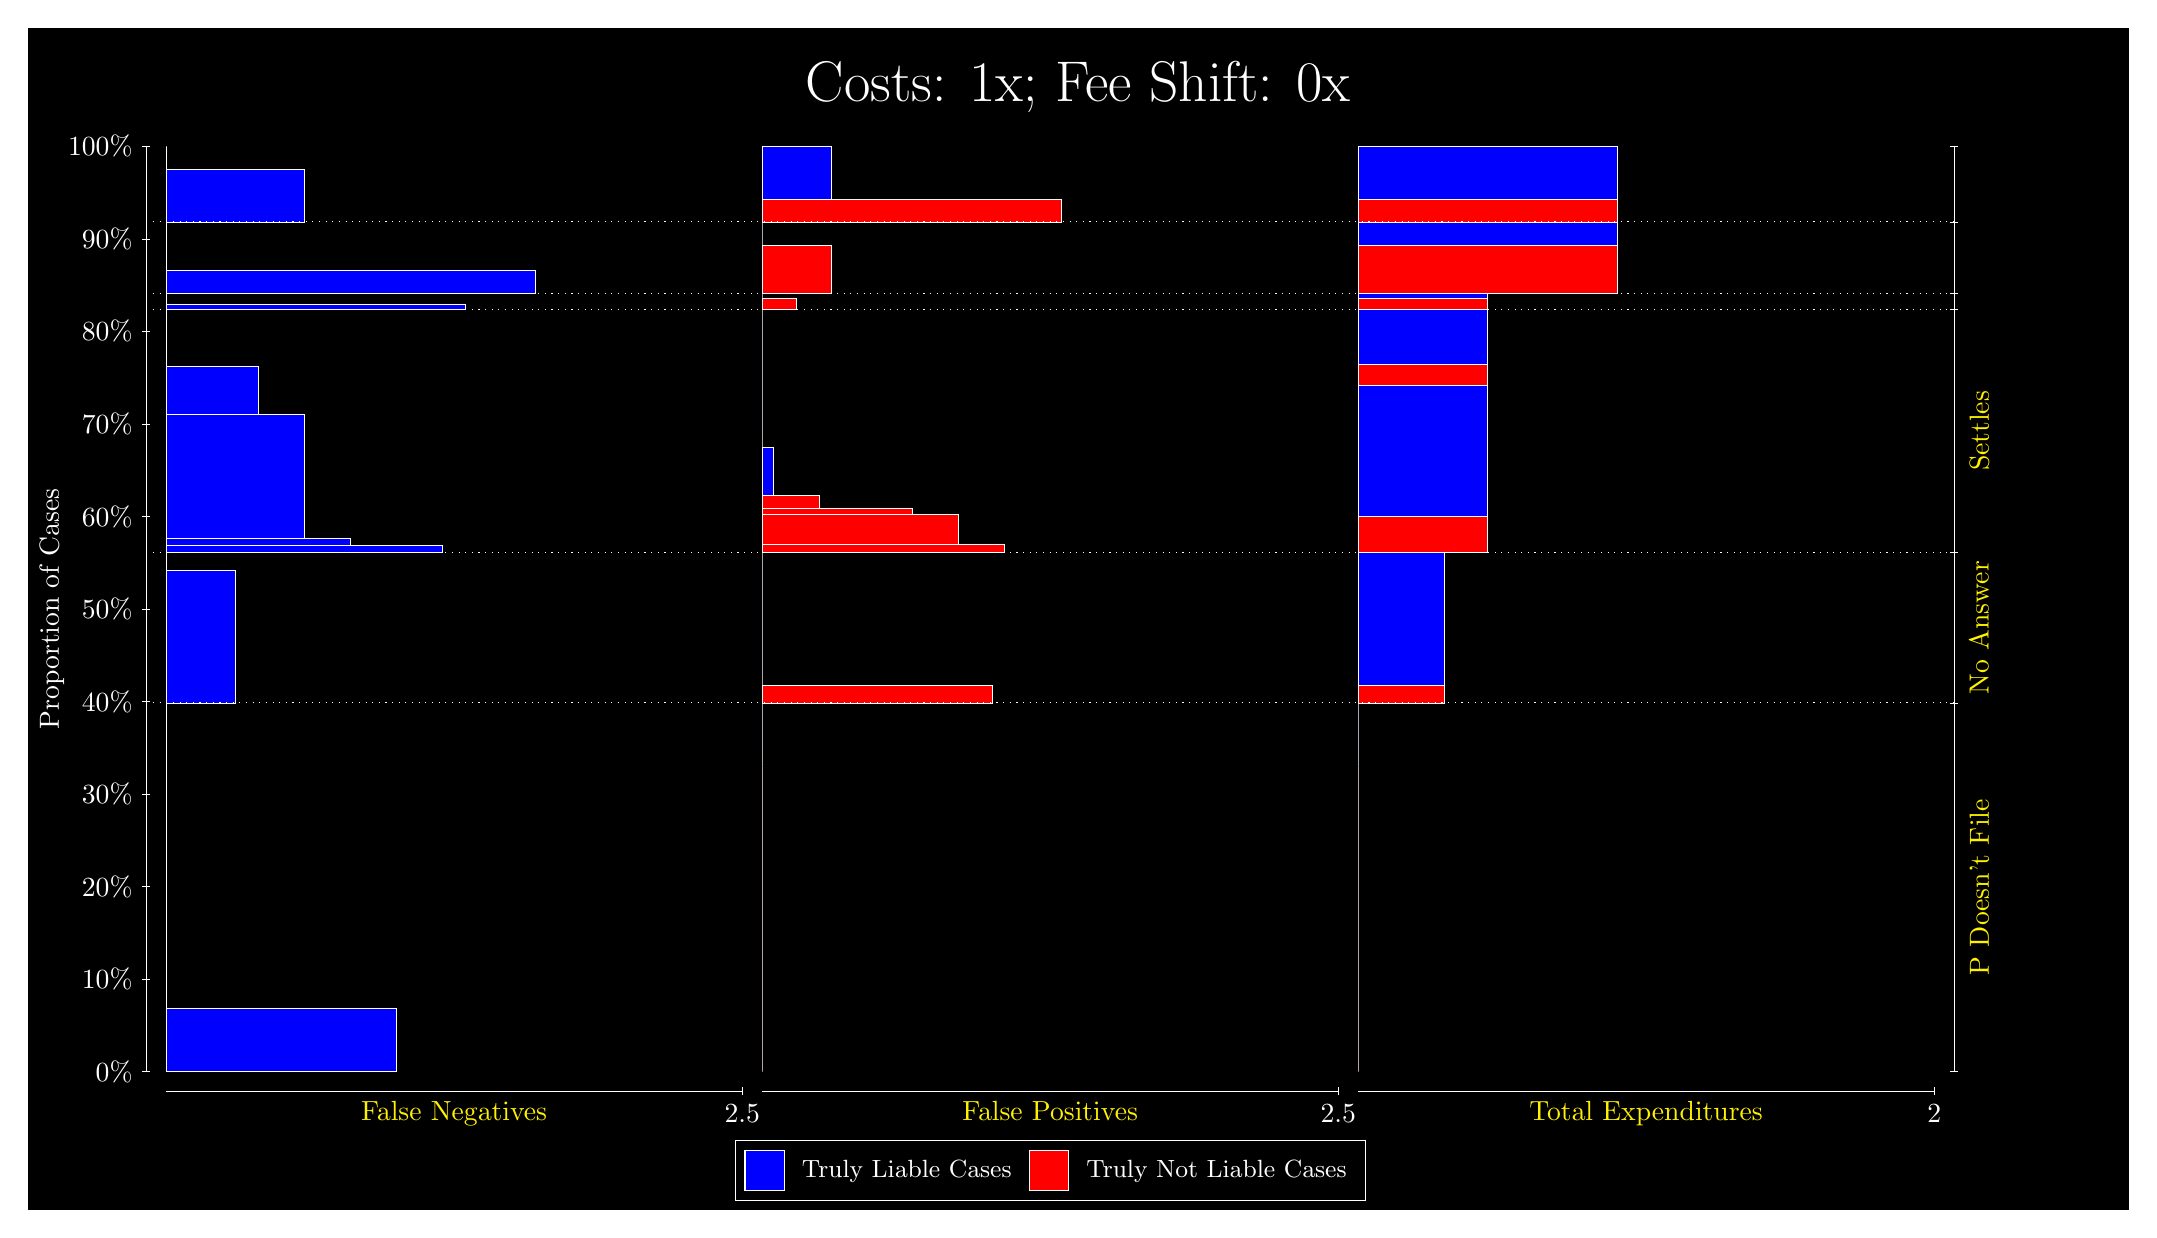
\begin{tikzpicture}
\draw[fill=black] (0,0) rectangle (26.667,15);
\draw[text=white] (0,13.5) rectangle (26.667,15) node[midway] {\huge Costs: 1x; Fee Shift: 0x};
\draw[white, very thin] (1.5,1.75) -- (1.5,13.5);
\node[rotate=90, text=white, anchor=center] at (0.3, 7.625) {Proportion of Cases};
\draw[white, very thin] (1.45,1.75) -- (1.55,1.75);
\node[text=white, anchor=east] at (1.45, 1.75) {0\%};
\draw[white, very thin] (1.45,2.925) -- (1.55,2.925);
\node[text=white, anchor=east] at (1.45, 2.925) {10\%};
\draw[white, very thin] (1.45,4.1) -- (1.55,4.1);
\node[text=white, anchor=east] at (1.45, 4.1) {20\%};
\draw[white, very thin] (1.45,5.275) -- (1.55,5.275);
\node[text=white, anchor=east] at (1.45, 5.275) {30\%};
\draw[white, very thin] (1.45,6.45) -- (1.55,6.45);
\node[text=white, anchor=east] at (1.45, 6.45) {40\%};
\draw[white, very thin] (1.45,7.625) -- (1.55,7.625);
\node[text=white, anchor=east] at (1.45, 7.625) {50\%};
\draw[white, very thin] (1.45,8.8) -- (1.55,8.8);
\node[text=white, anchor=east] at (1.45, 8.8) {60\%};
\draw[white, very thin] (1.45,9.975) -- (1.55,9.975);
\node[text=white, anchor=east] at (1.45, 9.975) {70\%};
\draw[white, very thin] (1.45,11.15) -- (1.55,11.15);
\node[text=white, anchor=east] at (1.45, 11.15) {80\%};
\draw[white, very thin] (1.45,12.325) -- (1.55,12.325);
\node[text=white, anchor=east] at (1.45, 12.325) {90\%};
\draw[white, very thin] (1.45,13.5) -- (1.55,13.5);
\node[text=white, anchor=east] at (1.45, 13.5) {100\%};

\draw[white, very thin] (24.457,1.75) -- (24.457,13.5);
\draw[white, very thin] (24.407,1.75) -- (24.507,1.75);
\node[anchor=west] at (24.407, 1.75) {};
\draw[white, very thin] (24.407,6.4319) -- (24.507,6.4319);
\node[anchor=west] at (24.407, 6.4319) {};
\draw[white, very thin] (24.407,8.3409) -- (24.507,8.3409);
\node[anchor=west] at (24.407, 8.3409) {};
\draw[white, very thin] (24.407,11.431) -- (24.507,11.431);
\node[anchor=west] at (24.407, 11.431) {};
\draw[white, very thin] (24.407,11.629) -- (24.507,11.629);
\node[anchor=west] at (24.407, 11.629) {};
\draw[white, very thin] (24.407,12.54) -- (24.507,12.54);
\node[anchor=west] at (24.407, 12.54) {};
\draw[white, very thin] (24.407,13.5) -- (24.507,13.5);
\node[anchor=west] at (24.407, 13.5) {};

\draw[white, very thin, fill=blue] (1.75,1.75) rectangle (4.6775,2.5559);
\draw[white, very thin, fill=red] (1.75,2.5559) rectangle (1.75,6.4319);
\draw[white, very thin, fill=blue] (1.75,6.4319) rectangle (2.6283,8.1167);
\draw[white, very thin, fill=red] (1.75,8.1167) rectangle (1.75,8.3409);
\draw[white, very thin, fill=blue] (1.75,8.3409) rectangle (5.2631,8.4308);
\draw[white, very thin, fill=blue] (1.75,8.4308) rectangle (4.092,8.5234);
\draw[white, very thin, fill=blue] (1.75,8.5234) rectangle (3.5065,10.096);
\draw[white, very thin, fill=blue] (1.75,10.096) rectangle (2.921,10.706);
\draw[white, very thin, fill=red] (1.75,10.706) rectangle (1.75,11.431);
\draw[white, very thin, fill=blue] (1.75,11.431) rectangle (5.5558,11.491);
\draw[white, very thin, fill=red] (1.75,11.491) rectangle (1.75,11.629);
\draw[white, very thin, fill=blue] (1.75,11.629) rectangle (6.4341,11.921);
\draw[white, very thin, fill=red] (1.75,11.921) rectangle (1.75,12.54);
\draw[white, very thin, fill=blue] (1.75,12.54) rectangle (3.5065,13.208);
\draw[white, very thin, fill=red] (1.75,13.208) rectangle (1.75,13.5);
\draw[white, very thin, fill=red] (9.3189,1.75) rectangle (9.3189,5.626);
\draw[white, very thin, fill=blue] (9.3189,5.626) rectangle (9.3189,6.4319);
\draw[white, very thin, fill=red] (9.3189,6.4319) rectangle (12.246,6.6561);
\draw[white, very thin, fill=blue] (9.3189,6.6561) rectangle (9.3189,8.3409);
\draw[white, very thin, fill=red] (9.3189,8.3409) rectangle (12.393,8.4426);
\draw[white, very thin, fill=red] (9.3189,8.4426) rectangle (11.807,8.8238);
\draw[white, very thin, fill=red] (9.3189,8.8238) rectangle (11.222,8.9071);
\draw[white, very thin, fill=red] (9.3189,8.9071) rectangle (10.051,9.0663);
\draw[white, very thin, fill=blue] (9.3189,9.0663) rectangle (9.4652,9.6761);
\draw[white, very thin, fill=blue] (9.3189,9.6761) rectangle (9.3189,11.431);
\draw[white, very thin, fill=red] (9.3189,11.431) rectangle (9.758,11.569);
\draw[white, very thin, fill=blue] (9.3189,11.569) rectangle (9.3189,11.629);
\draw[white, very thin, fill=red] (9.3189,11.629) rectangle (10.197,12.248);
\draw[white, very thin, fill=blue] (9.3189,12.248) rectangle (9.3189,12.54);
\draw[white, very thin, fill=red] (9.3189,12.54) rectangle (13.125,12.832);
\draw[white, very thin, fill=blue] (9.3189,12.832) rectangle (10.197,13.5);
\draw[white, very thin, fill=red] (16.888,1.75) rectangle (16.888,5.626);
\draw[white, very thin, fill=blue] (16.888,5.626) rectangle (16.888,6.4319);
\draw[white, very thin, fill=red] (16.888,6.4319) rectangle (17.986,6.6561);
\draw[white, very thin, fill=blue] (16.888,6.6561) rectangle (17.986,8.3409);
\draw[white, very thin, fill=red] (16.888,8.3409) rectangle (18.534,8.8054);
\draw[white, very thin, fill=blue] (16.888,8.8054) rectangle (18.534,10.471);
\draw[white, very thin, fill=red] (16.888,10.471) rectangle (18.534,10.732);
\draw[white, very thin, fill=blue] (16.888,10.732) rectangle (18.534,11.431);
\draw[white, very thin, fill=red] (16.888,11.431) rectangle (18.534,11.569);
\draw[white, very thin, fill=blue] (16.888,11.569) rectangle (18.534,11.629);
\draw[white, very thin, fill=red] (16.888,11.629) rectangle (20.181,12.248);
\draw[white, very thin, fill=blue] (16.888,12.248) rectangle (20.181,12.54);
\draw[white, very thin, fill=red] (16.888,12.54) rectangle (20.181,12.832);
\draw[white, very thin, fill=blue] (16.888,12.832) rectangle (20.181,13.5);
\draw[white, dotted] (1.5,6.4319) -- (24.457,6.4319);
\draw[white, dotted] (1.5,8.3409) -- (24.457,8.3409);
\draw[white, dotted] (1.5,11.431) -- (24.457,11.431);
\draw[white, dotted] (1.5,11.629) -- (24.457,11.629);
\draw[white, dotted] (1.5,12.54) -- (24.457,12.54);
\draw[white, very thin] (1.75,1.5) -- (9.0689,1.5);
\node[text=yellow, anchor=north] at (5.4094, 1.5) {False Negatives};
\draw[white, very thin] (9.0689,1.45) -- (9.0689,1.55);
\node[text=white, anchor=north] at (9.0689, 1.45) {2.5};

\draw[white, very thin] (9.3189,1.5) -- (16.638,1.5);
\node[text=yellow, anchor=north] at (12.978, 1.5) {False Positives};
\draw[white, very thin] (16.638,1.45) -- (16.638,1.55);
\node[text=white, anchor=north] at (16.638, 1.45) {2.5};

\draw[white, very thin] (16.888,1.5) -- (24.207,1.5);
\node[text=yellow, anchor=north] at (20.547, 1.5) {Total Expenditures};
\draw[white, very thin] (24.207,1.45) -- (24.207,1.55);
\node[text=white, anchor=north] at (24.207, 1.45) {2};

\node[text=yellow, centered, rotate=90] at (24.777, 4.091) {P Doesn't File};
\node[text=yellow, centered, rotate=90] at (24.777, 7.3864) {No Answer};
\node[text=yellow, centered, rotate=90] at (24.777, 9.8862) {Settles};




\draw (12.978300999999998,1.5) node[draw=none] (baseCoordinate) {};
\begin{scope}[align=center]
        \matrix[scale=0.5, draw=white, below=0.5cm of baseCoordinate, nodes={draw}, column sep=0.1cm]{
            \node[rectangle, draw, minimum width=0.5cm, minimum height=0.5cm, fill=blue] {}; &
            \node[draw=none, font=\small, text=white] (B) {Truly Liable Cases}; &
            \node[rectangle, draw, minimum width=0.5cm, minimum height=0.5cm, fill=red] {}; &
            \node[draw=none, font=\small, text=white] (B) {Truly Not Liable Cases}; \\
            };
\end{scope}

\end{tikzpicture}
\end{document}